% !TeX root = RJwrapper.tex
\title{ML Assignment 2: NHANES data}
\author{by Imran Aziz, Conrard G. T. Feugmo, Andre Schardong, Milton Segura, Sarpreet Gill}

\maketitle


% Any extra LaTeX you need in the preamble

\newpage

\hypertarget{introduction}{%
\section{Introduction:}\label{introduction}}

The following is a hypothetical business problem: A pharmaceutical
company is looking to better understand what the data related to
subjects and various health conditions and miscellaneous attributes.

\begin{itemize}
\item
  \textbf{Terms}

  \textbf{Subject} - is a person who has been surveyed by the NHMS
  dataset for various attributes related to the following: demographics,
  examinations, dietary, questionnaire(medical conditions), and
  medication

  \textbf{Health Conditions} - various diseases or ailments that people
  may inhibit such as sleep disorders, diabetes, oral health,
  cholesterol.

  \textbf{The National Health and Nutrition Examination Survey (NHANES)}
  - is a program of studies designed to assess the health and
  nutritional status of adults and children in the
\item
  \textbf{Data Description}
\end{itemize}

The data is spread against 6 spreadsheets (CSV): Demographics,
Examinations, Dietary, Laboratory, Questionnaire, and Medication.

\hypertarget{business-case}{%
\section{Business Case}\label{business-case}}

A pharmaceutical company wants to produce new drugs. The company is
curious as to whether existing data on subjects and their associated
health conditions could provide advice and insight to their drug
researchers. They have obtained NHMS dataset. This dataset contains
subject/patient data along with various information including health
conditions.

The company is interested in producing new drugs for the following
health conditions: diabetes and hypertension/cholesterol (we can add or
remove health conditions later. At the very least, let's keep diabetes
or something).

\hypertarget{first-problem}{%
\subsection{First Problem:}\label{first-problem}}

What types of symptoms, medications, diet, demographics are common among
various health conditions (such as diabetes)? For example, what types of
dietary factors are commonly found with diabetes?

\hypertarget{second-problem}{%
\subsection{Second Problem:}\label{second-problem}}

Are their any commonalities between various people with the same health
conditions? For example, if subject 1 and subject 2 have the same health
condition (for example, diabetes) what other similarities would these
subjects have?

They have approached our Machine Learning group for help on these
problems.

\hypertarget{analytical-reframing-for-the-business-case.}{%
\section{Analytical Reframing for the Business
Case.}\label{analytical-reframing-for-the-business-case.}}

The first business problem involves using ``health condition'' features
and finding related features. This is an association problem and we will
need a model using an association algorithm. What features are
associated with ``health condition'' features? We're comparing the rows
of the dataset.

The second business problem involves finding commonality between
subjects. This is a clustering problem and we will need a model using a
clustering algorithm. We need to determine whether business's
presumption is accurate: Can subjects be divided into discrete groups
according to their health conditions, which could then provide
meaningful data for the drug researchers? If yes, we need to find these
clusters of subjects that can be used to segregate the data by health
conditions, then we can report these findings to the business. Or is
there too much commonality between ``health condition'' features and
other features? If we cannot find clusters that could be divided by
health conditions, then we will also report this finding to the company
as well and note that clusters that we did find. We're comparing the
columns/attributes of the dataset.

\hypertarget{how-do-we-define-health-conditions-within-the-dataset}{%
\subsection{How do we define health conditions within the dataset
?}\label{how-do-we-define-health-conditions-within-the-dataset}}

How do we know what is considered a health condition within the data? We
could use lab data and diagnose whether someone falls under the
definition of health condition; however, for the purpose

Diabetes within Questionnaire dataset:

We are postulating that the following features/columns indicate that an
individual has diabetes

DID040 - ``How old \{was SP/were you\} when a doctor or other health
professional first told \{you/him/her\} that \{you/he/she\} had diabetes
or sugar diabetes?''

DID060 - ``For how long \{have you/has SP\} been taking insulin?''

NA in the above features might indicate the subject does not have
diabetes.

For the association problem, we will need to see which attributes are
tied to above features.

Blood Pressure within Questionnaire dataset

BPD035 - How old \{were you/was SP\} when \{you were/he/she was\} first
told that \{you/he/she\} had hypertension or high blood pressure?

BPQ020 - \{Have you/Has SP\} ever been told by a doctor or other health
professional that \{you/s/he\} had hypertension, also called high blood
pressure?

Cancer

MCQ220 - \{Have you/Has SP\} ever been told by a doctor or other health
professional that \{you/s/he\} had cancer or a malignancy
(ma-lig-nan-see) of any kind?

\hypertarget{loading-r-packages}{%
\section{Loading R packages}\label{loading-r-packages}}

\begin{Schunk}
\begin{Sinput}
library(plyr)
library(dplyr)
library(tidyr)
library(ggplot2)
library(knitr)
\end{Sinput}
\end{Schunk}

\hypertarget{data-exploration}{%
\section{Data Exploration}\label{data-exploration}}

\begin{Schunk}
\begin{Sinput}
# Reading files
demographic   = read.csv("Data/Raw/demographic.csv", header = TRUE, na.strings = c("NA","","#NA"))
diet          = read.csv("Data/Raw/diet.csv", header = TRUE, na.strings = c("NA","","#NA"))
examination   = read.csv("Data/Raw/examination.csv", header = TRUE, na.strings = c("NA","","#NA"))
labs          = read.csv("Data/Raw/labs.csv", header = TRUE, na.strings = c("NA","","#NA"))
medications   = read.csv("Data/Raw/medications.csv", header = TRUE, na.strings = c("NA","","#NA"))
questionnaire = read.csv("Data/Raw/questionnaire.csv", header = TRUE, na.strings = c("NA","","#NA"))

# Merging files
data_List = list(demographic,examination,diet,labs,questionnaire,medications)
Data_joined = join_all(data_List) #require(plyr)
\end{Sinput}
\end{Schunk}

\hypertarget{checking-for-missing-data}{%
\subsection{Checking for missing data}\label{checking-for-missing-data}}

Its always important to check for missing values and consider how to fix
them.

\begin{itemize}
\tightlist
\item
  \textbf{Demographic}
\end{itemize}

\begin{Schunk}
\begin{Sinput}
#library(knitr)
knitr::include_graphics("Figures/demographic_MS.png")
\end{Sinput}


\begin{center}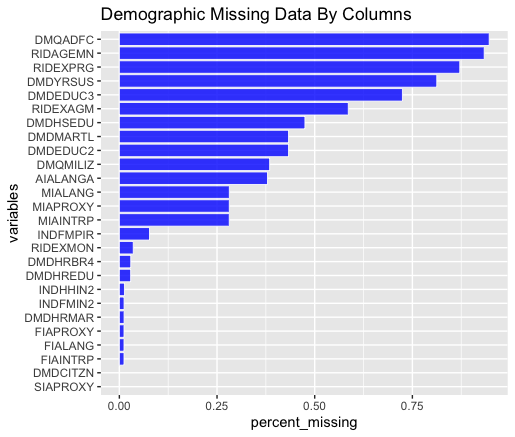
\includegraphics[width=7.15in]{Figures/demographic_MS} \end{center}

\end{Schunk}

\begin{itemize}
\tightlist
\item
  \textbf{Medications}
\end{itemize}

\begin{Schunk}
\begin{Sinput}
#library(knitr)
knitr::include_graphics("Figures/medications_MS.png")
\end{Sinput}


\begin{center}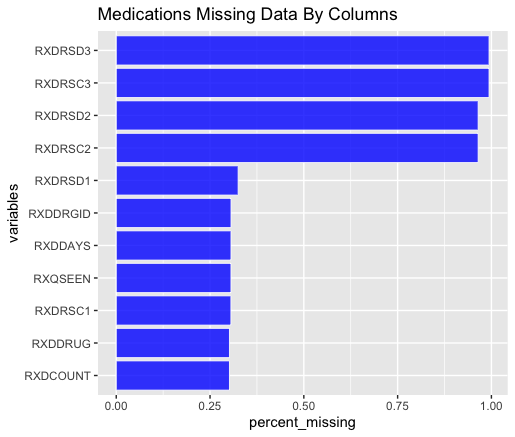
\includegraphics[width=7.15in]{Figures/medications_MS} \end{center}

\end{Schunk}

\begin{itemize}
\tightlist
\item
  \textbf{Others spreadsheets }
\end{itemize}

We did represent the rest of spreadsheets because the percentage of
missing data are very important. Just for example

\begin{Schunk}
\begin{Sinput}
#library(knitr)
knitr::include_graphics("Figures/examination_MS.png")
\end{Sinput}


\begin{center}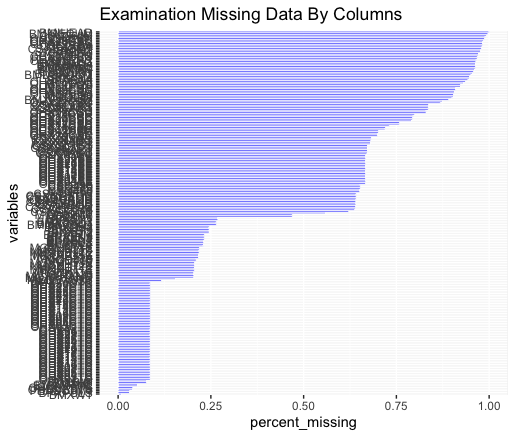
\includegraphics[width=7.15in]{Figures/examination_MS} \end{center}

\end{Schunk}

\hypertarget{data-splitting-imputation}{%
\subsection{Data splitting \&
imputation}\label{data-splitting-imputation}}

There are many ways to do data imputation, but random forest imputation
will be used since it is robust and reliable method.

\hypertarget{visualising-all-numeric-columns}{%
\subsection{Visualising all numeric
columns}\label{visualising-all-numeric-columns}}

It is useful to show histograms of all numeric columns.

\hypertarget{visualising-correlation}{%
\subsection{Visualising correlation}\label{visualising-correlation}}

\hypertarget{exploring-by-location}{%
\subsection{Exploring by location}\label{exploring-by-location}}

\hypertarget{exploring-by-age}{%
\subsection{Exploring by age}\label{exploring-by-age}}

\hypertarget{problem-1-clustering}{%
\section{Problem 1: Clustering}\label{problem-1-clustering}}

\hypertarget{pca}{%
\subsection{PCA}\label{pca}}

\hypertarget{k-means}{%
\subsection{K-means}\label{k-means}}

\hypertarget{hierarchical-agglomerative}{%
\subsection{Hierarchical
Agglomerative}\label{hierarchical-agglomerative}}

\hypertarget{summary-of-models}{%
\subsection{Summary of models}\label{summary-of-models}}

\hypertarget{problem-2-association}{%
\section{Problem 2: Association}\label{problem-2-association}}


\address{%
Imran Aziz\\
\\
\\
}


\address{%
Conrard G. T. Feugmo\\
\\
\\
}


\address{%
Andre Schardong\\
\\
\\
}


\address{%
Milton Segura\\
\\
\\
}


\address{%
Sarpreet Gill\\
York University School of Continuing Studies\\
\\
}


